\documentclass{article}
\usepackage{graphicx}
\usepackage[boxruled,linesnumbered]{algorithm2e} 
\usepackage[
top    = 2.5cm,
bottom = 2.5cm,
left   = 3.50cm,
right  = 2.50cm]{geometry}

\begin{document}
\title{Experimental Results}
\date{}
\maketitle

We have compared all the results with the respective serial algorithms. We have tested all the implementations on two machines. Description of machines is as follows :

\begin{enumerate}
\item \textbf{Machine 1} 
\begin{itemize}
\item \textbf{Processor Name} : Intel(R) Core(TM) i7-4770  
\item \textbf{No of Cores} : 4
\item \textbf{Threads per core} : 2
\item \textbf{Cache}
\begin{itemize}
\item L1 = 32KB
\item L2 = 256 KB
\item L3 = 8 MB
\end{itemize}
\end{itemize}

\item \textbf{Machine 2}
\begin{itemize}
\item \textbf{Processor Name} : Intel(R) Xeon(R)  E5-2670  
\item \textbf{No of Cores} : 16
\item \textbf{Threads per core} : 2
\item \textbf{Cache}
\begin{itemize}
\item L1 = 32KB
\item L2 = 256 KB
\item L3 = 20 MB
\end{itemize}
\end{itemize}

\end{enumerate}


\section{Breadth First Search (BFS)}
We have tested this algorithm on 4 graph datasets. For large graph cilk plus implementation shows the speedup over the serial implementation, but for smaller graph cilk plus implementation takes more time than serial implementation. In smaller graph, \textbf{Cilk Plus Reducer List} overhead is more than the parallel work. Reducer List takes more time if number of processors are less. \\

We have tested results on 4 dataset. Description of datasets are as follows.
\subsection{List of Graph Dataset}
\begin{enumerate}
\item \textbf{rmat22}
\begin{itemize}
\item Number of nodes = 4194304
\item Number of edges = 33226138
\end{itemize} 

\item \textbf{rmat20}
\begin{itemize}
\item Number of nodes = 1048576
\item Number of edges = 8259994
\end{itemize} 

\item \textbf{r4-2e23}
\begin{itemize}
\item Number of nodes = 8388608
\item Number of edges = 33554432
\end{itemize} 

\item \textbf{USA}
\begin{itemize}
\item Number of nodes = 264346
\item Number of edges = 730100
\end{itemize} 

\end{enumerate}

\begin{figure}
   \centering
   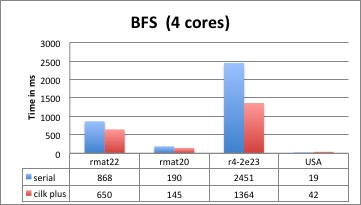
\includegraphics[width=7.0in]{bfs4}
   \caption{BFS results on 4 cores machine}
   \label{graph:bfs4}
\end{figure}

\begin{figure}
   \centering
   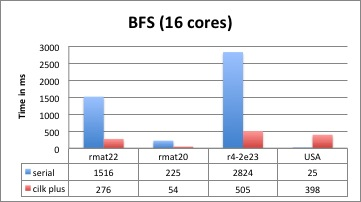
\includegraphics[width=7.0in]{bfs16}
   \caption{BFS results on 16 cores machine}
   \label{graph:bfs16}
\end{figure}



\subsection{Analysis}
Figure \ref{graph:bfs4} and figure \ref{graph:bfs16} shows results on 4 core machine and 16 core machine respectively. Graph 1 and 2 are sparse graph. It shows 1.33x and 1.31x speedup on 4 cores, 5.65x and 4.16x on 16 cores machine for these graphs respectively. Graph 3 is dense graph, so it has more scope for parallelism. Cilk Plus implementation shows 1.8x speedup on 4 cores machine and 5.6x speedup on 16 cores machine. Gprah 4 is a smaller graph. Because of reducer list overhead, cilk plus implementation performs slower than the serial implementation. 

%--------------------------------------------------------------------------

\section{Single Source Shortest Path (SSSP)}
We have tested this algorithm on 4 graph datasets as mentioned above. For large graph cilk plus implementation shows the speedup over the serial implementation, but for smaller graphs cilk plus implementation takes more time than serial implementation. In smaller graph, \textbf{Cilk Plus Reducer List} overhead is more than the parallel work. Reducer List takes more time if number of processors are less. \\



\begin{figure}
   \centering
   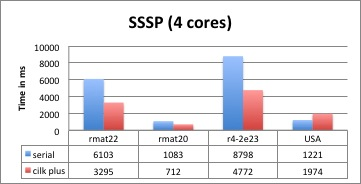
\includegraphics[width=7.0in]{sssp4}
   \caption{SSSP results on 4 cores machine}
   \label{graph:sssp4}
\end{figure}

\begin{figure}
   \centering
   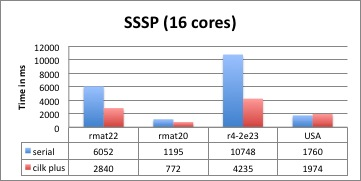
\includegraphics[width=7.0in]{sssp16}
   \caption{SSSP results on 16 cores machine}
   \label{graph:sssp16}
\end{figure}

\subsection{Analysis}

Figure \ref{graph:sssp4} and figure \ref{graph:sssp16} shows results on 4 core machine and 16 core machine respectively. Graph 1 and 2 are sparse graph. It shows 1.8x and 1.5x speedup on 4 cores, 2.13x and 1.54x on 16 cores machine for these graphs respectively. Graph 3 is dense graph, so it has more scope for parallelism. Cilk Plus implementation shows 1.8x speedup on 4 cores machine and 2.5x speedup on 16 cores machine. Gprah 4 is a smaller graph. Because of reducer list overhead, cilk plus implementation performs slower than the serial implementation. 



\end{document}